\documentclass[12pt,a4paper]{article}

\usepackage[utf8]{inputenc}
\usepackage[T1]{fontenc}
\usepackage{lmodern}
\usepackage{amsmath,amssymb,amsfonts}
\usepackage{graphicx}
\usepackage{float}
\usepackage[hidelinks]{hyperref}
\usepackage{geometry}
\usepackage{xcolor}
\usepackage{tcolorbox}
\usepackage{titlesec}
\usepackage{enumitem}
\usepackage{booktabs}
\usepackage{tikz}
\usetikzlibrary{arrows.meta,positioning,calc,shapes.geometric,decorations.pathmorphing,patterns}

\geometry{margin=1in}

\definecolor{softblue}{RGB}{232,244,255}
\definecolor{softyellow}{RGB}{255,251,230}
\definecolor{softgreen}{RGB}{239,252,242}
\definecolor{softrose}{RGB}{255,240,244}
\definecolor{ink}{RGB}{45,52,60}
\definecolor{gridblue}{RGB}{48,109,184}
\definecolor{warmorange}{RGB}{210,122,35}
\definecolor{deepgreen}{RGB}{45,135,90}

\newtcolorbox{definitionbox}{
  colback=softgreen,
  colframe=deepgreen!75!black,
  boxrule=0.5pt,
  arc=2mm,
  left=6pt,right=6pt,top=6pt,bottom=6pt
}
\newtcolorbox{formulabox}{
  colback=softyellow,
  colframe=warmorange!80!black,
  boxrule=0.5pt,
  arc=2mm,
  left=6pt,right=6pt,top=6pt,bottom=6pt
}
\newtcolorbox{theorembox}{
  colback=softblue,
  colframe=gridblue!80!black,
  boxrule=0.5pt,
  arc=2mm,
  left=6pt,right=6pt,top=6pt,bottom=6pt
}
\newtcolorbox{importantbox}{
  colback=softrose,
  colframe=red!45!black,
  boxrule=0.5pt,
  arc=2mm,
  left=6pt,right=6pt,top=6pt,bottom=6pt
}

\titleformat{\section}{\normalfont\Large\bfseries}{\thesection}{1em}{}
\titleformat{\subsection}{\normalfont\large\bfseries}{\thesubsection}{1em}{}
\titleformat{\subsubsection}{\normalfont\normalsize\bfseries}{\thesubsubsection}{1em}{}

\newcommand{\halfplane}{
\begin{scope}
\fill[blue!4] (-2.2,0) rectangle (2.2,1.65);
\draw[->,thick] (-2.35,0) -- (2.45,0) node[right] {$\Re z$};
\draw[->,thick] (0,-0.25) -- (0,1.85) node[above] {$\Im z$};
\foreach \x/\lab in {-1.6/$x_1$,-0.6/$x_2$,0.55/$x_3$,1.65/$x_4$}{
  \filldraw[red!70!black] (\x,0) circle (2pt) node[below=4pt] {\lab};
}
\node at (0,1.35) {upper half-plane};
\end{scope}
}

\begin{document}

\pagenumbering{arabic}

\begin{center}
\vspace*{1.8cm}
{\fontsize{16}{19}\selectfont\textbf{Computation of Conformal Mappings}}

\vspace{0.35cm}
{\large\textbf{Final Report on Schwarz-Christoffel Integrals and Numerical Methods}}

\vspace{1cm}
Final Project Report submitted to

\vspace{0.3cm}
\textbf{Indian Institute of Technology Kharagpur}

\vspace{1.3cm}
In partial fulfilment of the requirements for the award of the degree of

\vspace{0.3cm}
B.S.(Hons.) in Mathematics and Computing

\vspace{0.5cm}
By

\vspace{0.3cm}
\textbf{Ravi Kumar}

\vspace{0.2cm}
\textbf{22MA10047}

\vspace{0.9cm}
Under the guidance of

\vspace{0.3cm}
\textbf{Prof. Bappaditya Bhowmik}

\vspace{0.9cm}

\includegraphics[width=4.8cm]{../BTP-1/Images/IIT_Kharagpur_Logo.png}

\vspace{0.7cm}
\textbf{DEPARTMENT OF MATHEMATICS}

\textbf{INDIAN INSTITUTE OF TECHNOLOGY KHARAGPUR}

\vspace{0.45cm}
\textbf{April 2026}

\vspace{0.45cm}
\copyright\ 2026, Ravi Kumar. All rights reserved.
\end{center}

\newpage

\begin{center}
\textbf{\underline{DECLARATION}}
\end{center}
\vspace{2cm}

I certify that
\vspace{1cm}

\begin{enumerate}[label=\alph*., leftmargin=2cm]
\item the work contained in this report is original and has been done by me under the guidance of my supervisor(s).
\item the work has not been submitted to any other Institute for any degree or diploma.
\item I have followed the guidelines provided by the Institute in preparing the report.
\item I have conformed to the norms and guidelines given in the Ethical Code of Conduct of the Institute.
\item Whenever I have used material from other sources, I have cited the source in the report and listed it in the references.
\end{enumerate}

\vspace{3cm}
\hfill Signature of the Student

\newpage

\begin{center}
\textbf{\underline{CERTIFICATE}}
\end{center}
\vspace{2cm}

This is to certify that the report entitled, ``\textbf{Computation of Conformal Mappings: Final Report on Schwarz-Christoffel Integrals and Numerical Methods}'' submitted by \textbf{Mr. Ravi Kumar} to Indian Institute of Technology, Kharagpur, India, is a record of bonafide project work carried out by him under my supervision and guidance and is worthy of consideration for the award of the degree of B.S.(Hons.) in Mathematics and Computing of the Institute.

\vspace{4cm}
\noindent\rule{5cm}{0.4pt}

\noindent Prof. Bappaditya Bhowmik

\noindent Department of Mathematics

\noindent Supervisor

\vspace{1cm}
\noindent Date: April 2026

\newpage


\section*{Abstract}
\addcontentsline{toc}{section}{Abstract}

This report studies the computational side of conformal mapping, with emphasis on Schwarz-Christoffel integrals and the numerical parameter problem. The first phase of the project introduced conformal maps, analytic functions, and the Schwarz-Christoffel formula as an explicit construction for polygonal domains. The final phase develops the problem further: given a target polygon, how are its prevertices and constants determined, how are singular integrals evaluated, and how do extremal principles provide alternate numerical constructions? The report discusses Newton iteration for side-ratio equations, singularity removal, disk-based Schwarz-Christoffel algorithms, variational methods, and the Bergman kernel. All diagrams in the technical body are original schematic illustrations prepared for this final report.

\begin{figure}[H]
\centering
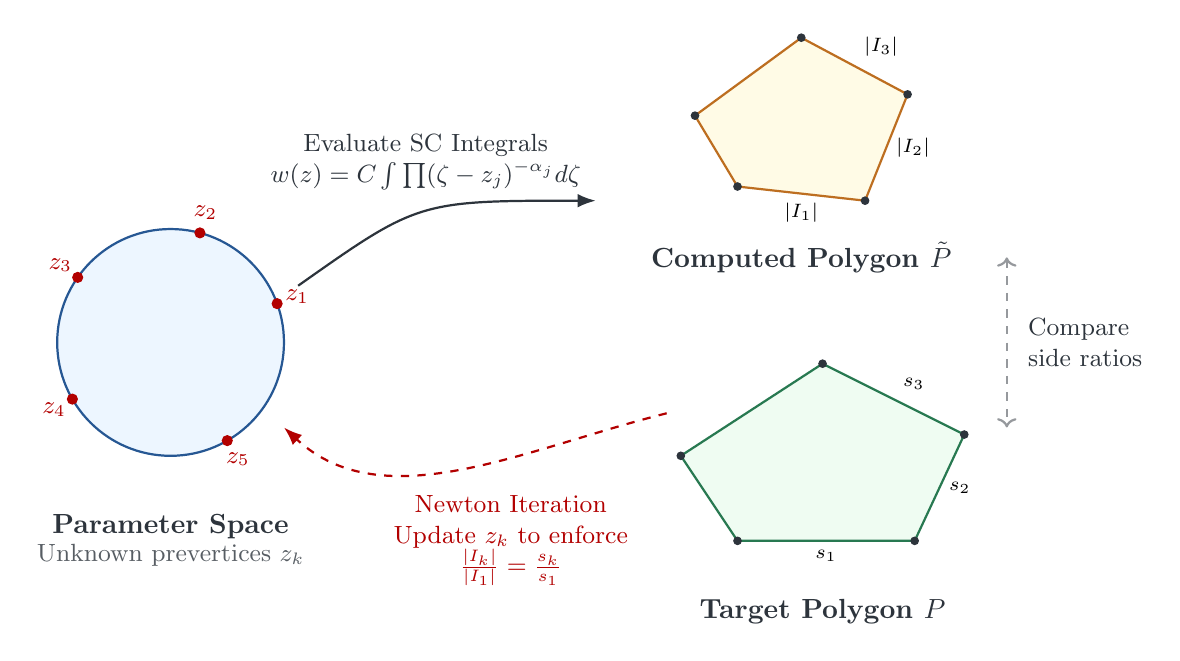
\begin{tikzpicture}[
  scale=0.9,
  node distance=1.5cm,
  arrow/.style={-Latex, thick, ink},
  update_arrow/.style={-Latex, dashed, thick, red!70!black}
]

% Prevertex Domain (Unit Disk)
\begin{scope}[xshift=0cm]
  \fill[softblue, opacity=0.8] (0,0) circle (1.6);
  \draw[thick, gridblue!80!black] (0,0) circle (1.6);
  \foreach \a/\k in {20/1, 75/2, 145/3, 210/4, 300/5}{
    \filldraw[red!70!black] (\a:1.6) circle (2pt);
    \node[font=\small, red!70!black] at (\a:1.9) {$z_\k$};
  }
  \node[font=\bfseries, ink] at (0,-2.6) {Parameter Space};
  \node[font=\small, ink!80] at (0,-3.0) {Unknown prevertices $z_k$};
\end{scope}

% Forward Map Arrow
\draw[arrow] (1.8, 0.8) .. controls (3.5, 2.0) .. (6.0, 2.0)
  node[midway, above, align=center, font=\small, yshift=4pt] {Evaluate SC Integrals\\$w(z) = C \int \prod (\zeta-z_j)^{-\alpha_j} d\zeta$};

% Computed Polygon (slightly distorted)
\begin{scope}[xshift=8.0cm, yshift=2.2cm]
  \coordinate (C1) at (0,0);
  \coordinate (C2) at (1.8,-0.2);
  \coordinate (C3) at (2.4, 1.3);
  \coordinate (C4) at (0.9, 2.1);
  \coordinate (C5) at (-0.6, 1.0);
  
  \draw[thick, fill=softyellow, draw=warmorange!90!black] (C1) -- (C2) -- (C3) -- (C4) -- (C5) -- cycle;
  \foreach \p in {C1,C2,C3,C4,C5} \filldraw[ink] (\p) circle (1.5pt);
  
  % Side labels (computed integrals)
  \node[below, font=\scriptsize] at (0.9,-0.1) {$|I_1|$};
  \node[right, font=\scriptsize] at (2.1, 0.55) {$|I_2|$};
  \node[above right, font=\scriptsize] at (1.65, 1.7) {$|I_3|$};
  
  \node[font=\bfseries, ink] at (0.9, -1.0) {Computed Polygon $\tilde{P}$};
\end{scope}

% Target Polygon (perfect)
\begin{scope}[xshift=8.0cm, yshift=-2.8cm]
  \coordinate (T1) at (0,0);
  \coordinate (T2) at (2.5, 0);
  \coordinate (T3) at (3.2, 1.5);
  \coordinate (T4) at (1.2, 2.5);
  \coordinate (T5) at (-0.8, 1.2);
  
  \draw[thick, fill=softgreen, draw=deepgreen!90!black] (T1) -- (T2) -- (T3) -- (T4) -- (T5) -- cycle;
  \foreach \p in {T1,T2,T3,T4,T5} \filldraw[ink] (\p) circle (1.5pt);
  
  % Side labels (target lengths)
  \node[below, font=\scriptsize] at (1.25, 0) {$s_1$};
  \node[right, font=\scriptsize] at (2.85, 0.75) {$s_2$};
  \node[above right, font=\scriptsize] at (2.2, 2.0) {$s_3$};
  
  \node[font=\bfseries, ink] at (1.2, -1.0) {Target Polygon $P$};
\end{scope}

% Comparison / Update Arrow
\draw[update_arrow] (7.0, -1.0) .. controls (5.0, -1.5) and (3.0, -2.5) .. (1.6, -1.2);
\node[align=center, font=\small, red!70!black] at (4.8, -2.8) {Newton Iteration\\Update $z_k$ to enforce\\$\frac{|I_k|}{|I_1|} = \frac{s_k}{s_1}$};

% Vertical comparison line
\draw[dashed, ink!50, <->, thick] (11.8, 1.2) -- (11.8, -1.2) node[midway, right=4pt, font=\small, align=left, ink] {Compare\\side ratios};

\end{tikzpicture}
\caption{The numerical parameter problem: computing prevertices $z_k$ such that the side lengths $|I_k|$ of the Schwarz-Christoffel map match the target side lengths $s_k$.}
\end{figure}

\newpage
\tableofcontents
\newpage

\section{Introduction}

Conformal mapping transforms one planar domain into another while preserving local angles. If \(w=f(z)\) is analytic and \(f'(z)\neq0\), then infinitesimal figures are rotated and scaled but not sheared. This makes conformal mapping particularly useful for two-dimensional potential problems, where the real and imaginary parts of analytic functions solve Laplace's equation.

The earlier part of this BTP established the basic framework: analytic functions, Cauchy--Riemann equations, the Riemann mapping theorem, bilinear transformations, and the Schwarz-Christoffel formula. This final report uses that foundation but shifts the focus from theory to computation. The main concern is the numerical construction of conformal maps for polygonal domains.

\begin{definitionbox}
A conformal map is locally equivalent to a rotation followed by a scaling. The scaling factor at \(z\) is \(|f'(z)|\), while the local rotation is \(\arg f'(z)\).
\end{definitionbox}

\section{Schwarz-Christoffel Mapping Revisited}

The Schwarz-Christoffel transformation maps a canonical domain, usually the upper half-plane or the unit disk, onto a polygonal domain. It is one of the few general formulas in conformal mapping that converts boundary geometry directly into an analytic expression. The key idea is simple: the real axis in the preimage plane is mapped to the polygon boundary, and each prevertex produces exactly the turn required at the corresponding polygon vertex.

\begin{figure}[H]
\centering
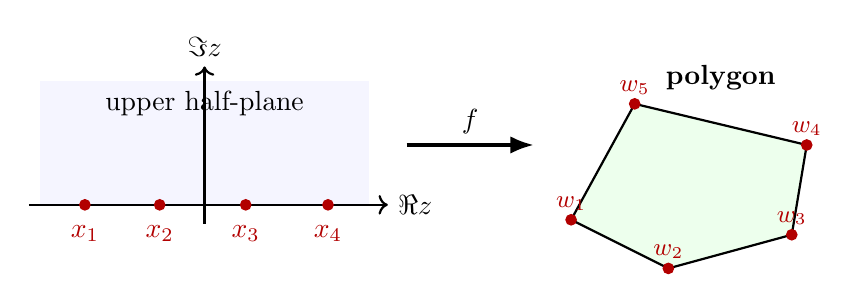
\begin{tikzpicture}[scale=0.95]
\halfplane
\begin{scope}[xshift=6.5cm]
\draw[thick,fill=green!7] (-1.6,-0.2) -- (-0.3,-0.85) -- (1.35,-0.4) -- (1.55,0.8) -- (-0.75,1.35) -- cycle;
\foreach \p/\lab in {(-1.6,-0.2)/$w_1$,(-0.3,-0.85)/$w_2$,(1.35,-0.4)/$w_3$,(1.55,0.8)/$w_4$,(-0.75,1.35)/$w_5$}{
  \filldraw[red!70!black] \p circle (2pt) node[font=\small,above] {\lab};
}
\node[font=\bfseries] at (0.4,1.7) {polygon};
\end{scope}
\draw[-Latex,very thick] (2.7,0.8) -- (4.4,0.8) node[midway,above] {$f$};
\end{tikzpicture}
\caption{Boundary correspondence: real prevertices \(x_k\) map to polygon vertices \(w_k\).}
\end{figure}

\subsection{Formula and Angle Data}

Let \(x_1<x_2<\cdots<x_n\) be prevertices on the real axis and let \(w_1,\ldots,w_n\) be the vertices of the polygon. If \(\theta_k\) is the interior angle at \(w_k\), define
\[
\alpha_k=1-\frac{\theta_k}{\pi}.
\]
The differential form of the upper half-plane Schwarz-Christoffel map is
\begin{formulabox}
\[
\frac{dw}{dz}=C_1\prod_{k=1}^{n}(z-x_k)^{-\alpha_k}.
\]
\end{formulabox}
Integrating gives the mapping function
\begin{formulabox}
\[
w(z)=C_1\int^z\prod_{k=1}^{n}(\zeta-x_k)^{-\alpha_k}\,d\zeta+C_2.
\]
\end{formulabox}
Here \(C_1\) fixes scale and rotation, while \(C_2\) fixes translation.

\begin{theorembox}
For a closed polygon,
\[
\theta_k=(1-\alpha_k)\pi,\qquad \sum_{k=1}^{n}\alpha_k=2.
\]
The sum condition is the analytic version of the fact that a closed polygon makes one full turn.
\end{theorembox}

\subsection{Argument Change at a Vertex}

The factor \((z-x_k)^{-\alpha_k}\) is responsible for the corner at \(w_k\). As \(z\) moves along the real axis and crosses \(x_k\) through the upper half-plane, the argument of \(z-x_k\) changes by \(-\pi\). Therefore
\[
\Delta\arg (z-x_k)^{-\alpha_k}
=-\alpha_k(-\pi)=\alpha_k\pi.
\]
This is precisely the exterior turning angle required at the polygon vertex. The product of all such factors places all the required turns into the derivative \(dw/dz\).

\begin{figure}[H]
\centering
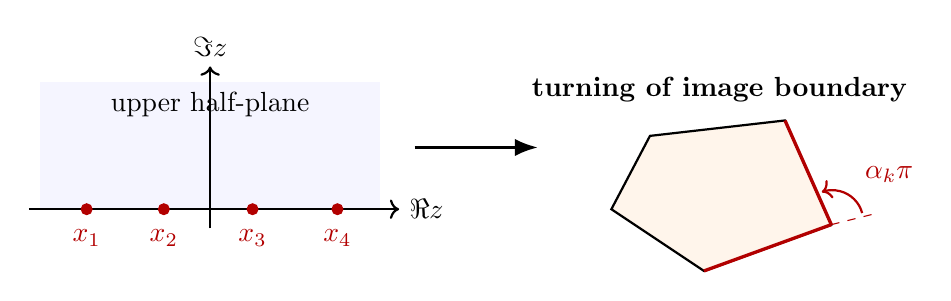
\begin{tikzpicture}[scale=0.98]
\halfplane
\begin{scope}[xshift=6.6cm]
\draw[thick, fill=orange!8] (-1.4,0) -- (-0.2,-0.8) -- (1.45,-0.2) -- (0.85,1.15) -- (-0.9,0.95) -- cycle;
\draw[very thick,red!70!black] (-0.2,-0.8) -- (1.45,-0.2);
\draw[very thick,red!70!black] (1.45,-0.2) -- (0.85,1.15);
\draw[dashed, red!70!black] (1.45,-0.2) -- (2.05,-0.05);
\draw[->,red!70!black,thick] (1.85,-0.05) arc (15:110:0.4);
\node[red!70!black] at (2.2,0.45) {$\alpha_k\pi$};
\node[font=\bfseries] at (0,1.55) {turning of image boundary};
\end{scope}
\draw[-Latex,very thick] (2.65,0.8) -- (4.25,0.8);
\end{tikzpicture}
\caption{Each factor \((z-x_k)^{-\alpha_k}\) produces the required boundary turn at a polygon vertex.}
\end{figure}

\subsection{Construction Procedure}

The practical construction of an SC map follows four steps:
\begin{enumerate}
\item List the polygon vertices \(w_1,\ldots,w_n\) in counterclockwise order.
\item Compute the angle parameters \(\alpha_k=1-\theta_k/\pi\).
\item Fix three prevertices using Möbius normalization and solve for the remaining prevertices from side-length ratios.
\item Determine \(C_1\) and \(C_2\) from one side length and one vertex location.
\end{enumerate}

\begin{figure}[H]
\centering
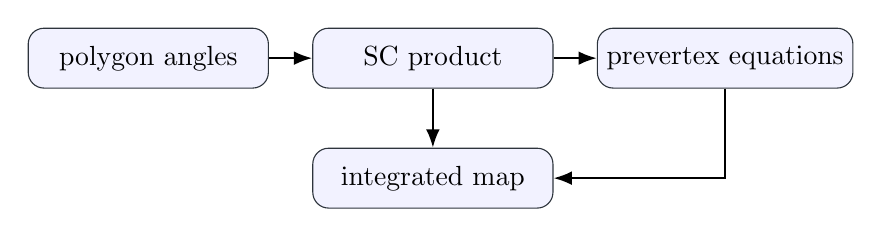
\begin{tikzpicture}[
  block/.style={rectangle,rounded corners=2mm,draw=ink,fill=blue!5,align=center,minimum width=3.05cm,minimum height=0.76cm},
  arrow/.style={-Latex,thick}
]
\node[block] (angles) {polygon angles};
\node[block,right=0.55cm of angles] (prod) {SC product};
\node[block,right=0.55cm of prod] (params) {prevertex equations};
\node[block,below=0.75cm of prod] (map) {integrated map};
\draw[arrow] (angles) -- (prod);
\draw[arrow] (prod) -- (params);
\draw[arrow] (params) |- (map);
\draw[arrow] (prod) -- (map);
\end{tikzpicture}
\caption{SC construction workflow from polygon geometry to mapping formula.}
\end{figure}

\subsection{Example Mappings}

\subsubsection{General Polygon}

For a general polygon with vertices \(w_1,w_2,\ldots,w_n\), the real axis is divided into intervals by the prevertices \(x_1,x_2,\ldots,x_n\). Each interval \([x_k,x_{k+1}]\) maps to one side of the polygon. Therefore, the side vector is given by
\begin{formulabox}
\[
w_{k+1}-w_k
=C_1\int_{x_k}^{x_{k+1}}
\prod_{j=1}^{n}(\zeta-x_j)^{-\alpha_j}\,d\zeta .
\]
\end{formulabox}
This equation is the geometric core of the Schwarz-Christoffel method: angles are determined by the exponents \(\alpha_j\), while side lengths are determined by the prevertex spacing.

\begin{figure}[H]
\centering
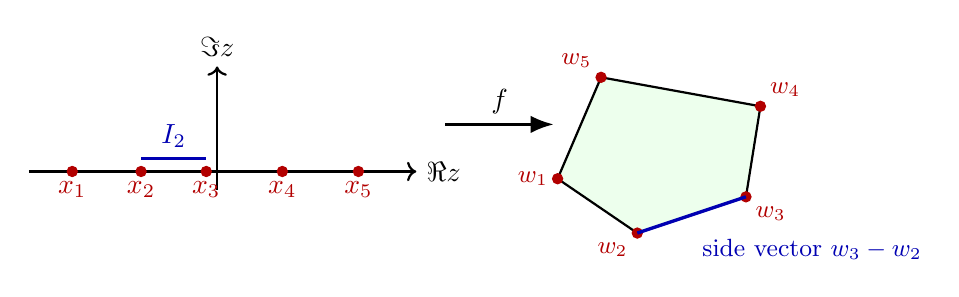
\begin{tikzpicture}[scale=0.92]
\draw[->,thick] (-2.6,0) -- (2.75,0) node[right] {$\Re z$};
\draw[->,thick] (0,-0.25) -- (0,1.45) node[above] {$\Im z$};
\foreach \x/\lab in {-2.0/$x_1$,-1.05/$x_2$,-0.15/$x_3$,0.9/$x_4$,1.95/$x_5$}{
  \filldraw[red!70!black] (\x,0) circle (2pt) node[below] {\lab};
}
\draw[very thick,blue!70!black] (-1.05,0.18) -- (-0.15,0.18) node[midway,above] {\(I_2\)};
\draw[-Latex,very thick] (3.15,0.65) -- (4.65,0.65) node[midway,above] {$f$};
\begin{scope}[xshift=6.05cm]
\draw[thick,fill=green!7] (-1.35,-0.1) -- (-0.25,-0.85) -- (1.25,-0.35) -- (1.45,0.9) -- (-0.75,1.3) -- cycle;
\foreach \p/\lab/\pos in {(-1.35,-0.1)/$w_1$/left,(-0.25,-0.85)/$w_2$/below left,(1.25,-0.35)/$w_3$/below right,(1.45,0.9)/$w_4$/above right,(-0.75,1.3)/$w_5$/above left}{
  \filldraw[red!70!black] \p circle (2pt) node[font=\small,\pos] {\lab};
}
\draw[very thick,blue!70!black] (-0.25,-0.85) -- (1.25,-0.35) node[midway,below right,yshift=-5pt,blue!70!black] {\small side vector $w_3-w_2$};
\end{scope}
\end{tikzpicture}
\caption{A prevertex interval in the upper half-plane maps to a corresponding polygon side.}
\end{figure}

\subsubsection{Disk to Triangle}

When the source domain is the unit disk instead of the upper half-plane, the Schwarz-Christoffel formula uses prevertices \(z_k=e^{i\Theta_k}\) on the unit circle \(|z|=1\). For a triangle the formula is
\begin{formulabox}
\[
w(z)=C_1\int_0^z
\prod_{k=1}^{3}(\zeta - z_k)^{-\alpha_k}\,d\zeta + C_2,
\qquad z_k = e^{i\Theta_k},\quad \alpha_k = 1-\frac{\theta_k}{\pi}.
\]
\end{formulabox}
Three prevertices on the circle can again be fixed by a Möbius normalization; for a triangle all three are fixed, so no nonlinear parameter problem remains. A convenient standard choice is
\[
z_1 = 1, \qquad z_2 = e^{2\pi i/3}, \qquad z_3 = e^{4\pi i/3}.
\]
For an equilateral target triangle (\(\alpha_k=2/3\) for all \(k\)) the integrand is \((z^3-1)^{-2/3}\) up to a constant, and the integral again reduces to a hypergeometric type.

\begin{figure}[H]
\centering
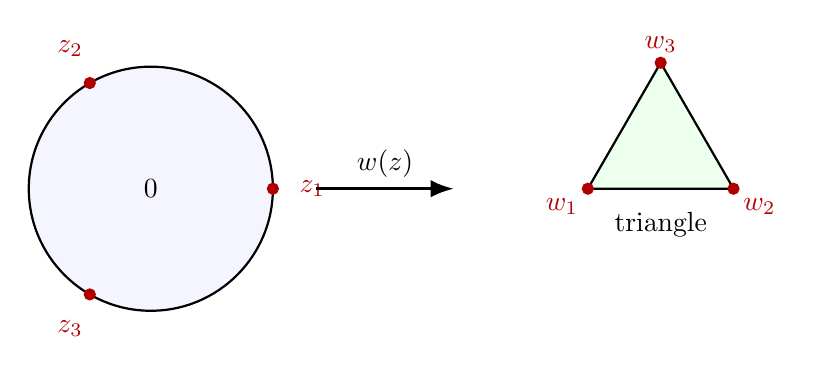
\begin{tikzpicture}[scale=1.0]
\draw[thick,fill=blue!4] (0,0) circle (1.55);
\node at (0,0) {$0$};
\foreach \a/\lab in {0/$z_1$,120/$z_2$,240/$z_3$}{
  \filldraw[red!70!black] (\a:1.55) circle (2pt) node at (\a:2.05) {\lab};
}
\draw[-Latex,very thick] (2.1,0) -- (3.85,0) node[midway,above] {$w(z)$};
\begin{scope}[xshift=5.55cm]
  \coordinate (A) at (0,0);
  \coordinate (B) at (1.85,0);
  \coordinate (C) at (0.925,1.6);
  \draw[thick,fill=green!7] (A) -- (B) -- (C) -- cycle;
  \filldraw[red!70!black] (A) circle (2pt) node[below left]  {$w_1$};
  \filldraw[red!70!black] (B) circle (2pt) node[below right] {$w_2$};
  \filldraw[red!70!black] (C) circle (2pt) node[above]       {$w_3$};
  \node at (0.925,-0.45) {triangle};
\end{scope}
\end{tikzpicture}
\caption{Disk to triangle: prevertices \(z_k\) placed symmetrically on \(|z|=1\) map to the vertices of the target triangle.}
\end{figure}

\subsubsection{Polygon to Triangle via Composition}

A direct conformal map from a general polygon \(P\) to a triangle \(T\) can be constructed by composing two SC maps:
\begin{enumerate}
  \item Map \(P\) to the upper half-plane \(\mathbb{H}\) via the \emph{inverse} SC map \(g:\,P\to\mathbb{H}\).
  \item Map \(\mathbb{H}\) to the triangle \(T\) via the SC map \(f:\,\mathbb{H}\to T\).
\end{enumerate}
The composed map \(f\circ g:\,P\to T\) is then a conformal bijection. In formula,
\begin{formulabox}
\[
\Phi = f\circ g : P \xrightarrow{\;g\;} \mathbb{H} \xrightarrow{\;f\;} T.
\]
\end{formulabox}
Neither \(f\) nor \(g\) has a compact closed form for a general polygon, but both can be evaluated numerically. The prevertex parameters for each stage are solved independently using the Newton iteration described in Section~4. After the two parameter problems are solved, function values of \(\Phi\) at interior points are obtained by numerical quadrature along a path from a known boundary point.

\begin{figure}[H]
\centering
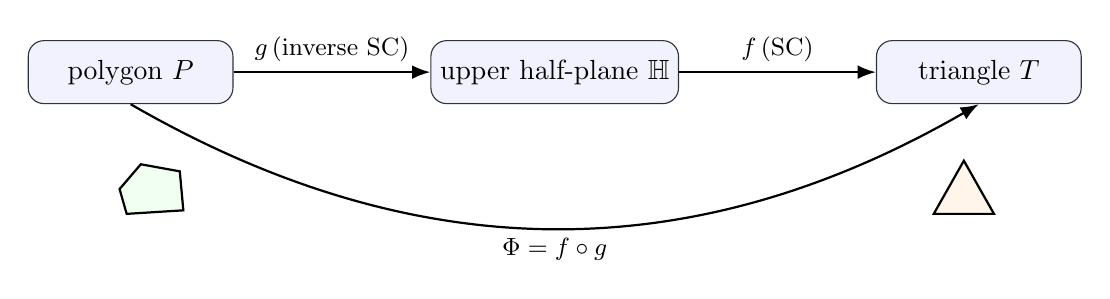
\begin{tikzpicture}[
  block/.style={rectangle,rounded corners=2mm,draw=ink,fill=blue!5,
                align=center,minimum width=2.6cm,minimum height=0.8cm},
  arrow/.style={-Latex,thick}
]
% polygon node
\node[block] (poly) {polygon $P$};
% half-plane node
\node[block,right=2.5cm of poly] (half) {upper half-plane $\mathbb{H}$};
% triangle node
\node[block,right=2.5cm of half] (tri) {triangle $T$};
% arrows
\draw[arrow] (poly) -- node[above,font=\small] {$g$\,(inverse SC)} (half);
\draw[arrow] (half) -- node[above,font=\small] {$f$\,(SC)} (tri);
% curved arrow under
\draw[arrow,bend right=30] (poly.south) to node[below,font=\small] {$\Phi=f\circ g$} (tri.south);
% small TikZ polygon sketch inside poly block vicinity
\begin{scope}[xshift=-0.05cm,yshift=-1.8cm,scale=0.45]
  \draw[thick,fill=green!6] (0,0)--(1.6,0.1)--(1.5,1.2)--(0.4,1.4)--(-0.2,0.7)--cycle;
\end{scope}
% small triangle sketch near tri block
\begin{scope}[xshift=10.2cm,yshift=-1.8cm,scale=0.45]
  \draw[thick,fill=orange!8] (0,0)--(1.7,0)--(0.85,1.5)--cycle;
\end{scope}
\end{tikzpicture}
\caption{Polygon to triangle via two-step composition: inverse SC maps \(P\) to \(\mathbb{H}\), then SC maps \(\mathbb{H}\) to \(T\).}
\end{figure}

\subsection{Why the Parameter Problem Appears}

The angles determine the exponents \(\alpha_k\), but they do not determine the side lengths. The relative side lengths depend on the prevertex spacing. Since real Möbius transformations preserve the upper half-plane, three prevertices may be fixed arbitrarily. The remaining \(n-3\) prevertices must be solved from side-ratio equations.

For adjacent vertices,
\[
w_{k+1}-w_k=C_1\int_{x_k}^{x_{k+1}}\prod_{j=1}^{n}(\zeta-x_j)^{-\alpha_j}\,d\zeta.
\]
Taking ratios removes the unknown scale \(|C_1|\), leaving nonlinear equations for the prevertices.

\begin{importantbox}
The practical obstacle in Schwarz-Christoffel mapping is not the formula itself; it is the coupled numerical determination of prevertices and the accurate evaluation of singular integrals.
\end{importantbox}

\section{Schwarz-Christoffel Integrals}

\subsection{Side Integrals}

The integrals between consecutive prevertices are called Schwarz-Christoffel integrals. A typical side integral is
\[
I_k=\int_{x_k}^{x_{k+1}}\prod_{j=1}^{n}(\zeta-x_j)^{-\alpha_j}\,d\zeta.
\]
The endpoints \(x_k\) and \(x_{k+1}\) are singular. For convex corners the singularities are integrable, but direct quadrature is inefficient unless the singular behavior is treated carefully.

\begin{figure}[H]
\centering
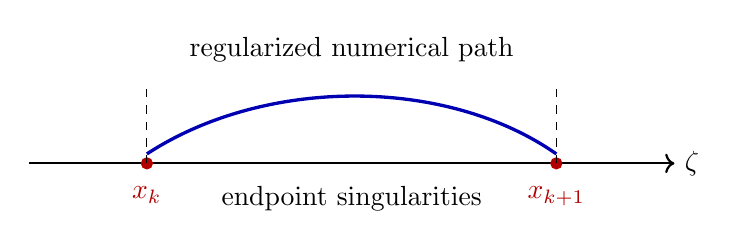
\begin{tikzpicture}[scale=1.0]
\draw[->,thick] (-0.5,0) -- (7.7,0) node[right] {$\zeta$};
\foreach \x/\lab in {1/$x_k$,6.2/$x_{k+1}$}{
  \filldraw[red!70!black] (\x,0) circle (2pt) node[below=5pt] {\lab};
}
\draw[blue!70!black,very thick] (1,0.12) .. controls (2.5,1.1) and (4.8,1.1) .. (6.2,0.12);
\draw[dashed] (1,0) -- (1,0.95);
\draw[dashed] (6.2,0) -- (6.2,0.95);
\node at (3.6,1.45) {regularized numerical path};
\node at (3.6,-0.45) {endpoint singularities};
\end{tikzpicture}
\caption{A side integral has singular behavior at both prevertices.}
\end{figure}

\subsection{Kantorovich-Type Singularity Removal}

Let the side integrand be written as
\[
F(\zeta)=(\zeta-x_k)^{-\alpha_k}(x_{k+1}-\zeta)^{-\alpha_{k+1}}\Phi(\zeta),
\]
where \(\Phi\) is smooth on the interval. The idea is to subtract the leading endpoint singular terms, integrate those analytically, and then apply ordinary quadrature to the smooth remainder:
\begin{align*}
F(\zeta)={}&(\zeta-x_k)^{-\alpha_k}A_k
+(x_{k+1}-\zeta)^{-\alpha_{k+1}}B_{k+1}
+R(\zeta).
\end{align*}
The constants \(A_k\) and \(B_{k+1}\) are chosen from local endpoint expansions. This improves numerical stability because \(R(\zeta)\) is much less singular than \(F(\zeta)\).

\begin{figure}[H]
\centering
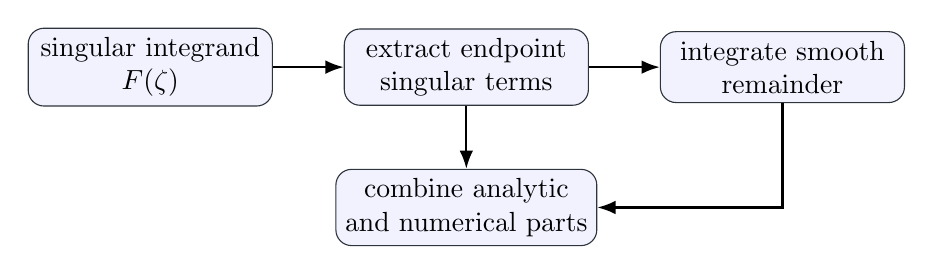
\begin{tikzpicture}[
  block/.style={rectangle,rounded corners=2mm,draw=ink,fill=blue!5,align=center,minimum width=3.1cm,minimum height=0.8cm},
  arrow/.style={-Latex,thick}
]
\node[block] (raw) {singular integrand\\\(F(\zeta)\)};
\node[block,right=0.9cm of raw] (split) {extract endpoint\\singular terms};
\node[block,right=0.9cm of split] (smooth) {integrate smooth\\remainder};
\node[block,below=0.8cm of split] (sum) {combine analytic\\and numerical parts};
\draw[arrow] (raw) -- (split);
\draw[arrow] (split) -- (smooth);
\draw[arrow] (smooth) |- (sum);
\draw[arrow] (split) -- (sum);
\end{tikzpicture}
\caption{Singularity-removal workflow for evaluating SC side integrals.}
\end{figure}

\section{Newton Method for the Parameter Problem}

For an \(n\)-sided polygon, the side lengths are controlled by the spacing of the prevertices. A real Möbius transformation maps the upper half-plane onto itself and can send any three real boundary points to any other three real boundary points. Therefore three prevertices may be fixed as a normalization, leaving \(n-3\) essential real unknowns. A common notation is
\[
X=(x_3,x_4,\ldots,x_{n-1}).
\]
Let the desired side-length ratios be
\[
\lambda_j=\frac{|w_{j+1}-w_j|}{|w_2-w_1|},\qquad j=2,\ldots,n-2.
\]
If \(I_j(X)\) denotes the SC integral over the \(j\)-th side interval, the parameter equations are
\[
I_j(X)=\lambda_j I_1(X),\qquad j=2,\ldots,n-2.
\]
It is convenient to write these as residual equations
\[
F_j(X)=I_j(X)-\lambda_j I_1(X),\qquad j=2,\ldots,n-2.
\]
The goal is to solve \(F(X)=0\).

\subsection{Linearization and Jacobian}

At an approximate solution \(X^{(m)}\), Newton's method linearizes the residual:
\[
F(X^{(m)}+h)\approx F(X^{(m)})+J(X^{(m)})h.
\]
The correction \(h^{(m)}\) is obtained from
\begin{formulabox}
\[
J(X^{(m)})h^{(m)}=-F(X^{(m)}),\qquad X^{(m+1)}=X^{(m)}+h^{(m)}.
\]
\end{formulabox}
The entries of the Jacobian are
\[
J_{j\nu}=\frac{\partial F_j}{\partial x_\nu}
=\frac{\partial I_j}{\partial x_\nu}
-\lambda_j\frac{\partial I_1}{\partial x_\nu},
\qquad \nu=3,\ldots,n-1.
\]
In practice these derivatives may be obtained analytically by differentiating the integrand with respect to the prevertices, or numerically by finite differences. Analytical derivatives are more accurate but require careful handling near singular endpoints; finite differences are simpler but can become unstable when prevertices are close together.

\subsection{Iteration and Stopping Criteria}

The Newton iteration is stopped when both the residual and the update are small, for example when
\[
\|F(X^{(m)})\|<\varepsilon_F
\quad \text{and}\quad
\|h^{(m)}\|<\varepsilon_X.
\]
The prevertices must remain ordered on the real axis. If a Newton step breaks the ordering or makes the residual larger, one uses a damped step
\[
X^{(m+1)}=X^{(m)}+\eta h^{(m)},\qquad 0<\eta\le 1,
\]
where \(\eta\) is reduced until the step is acceptable.

\begin{importantbox}
Newton's method is locally fast but not globally safe. It needs a reasonable initial guess, accurate quadrature for each SC integral, and safeguards when prevertices become crowded or nearly collide.
\end{importantbox}

\begin{figure}[H]
\centering
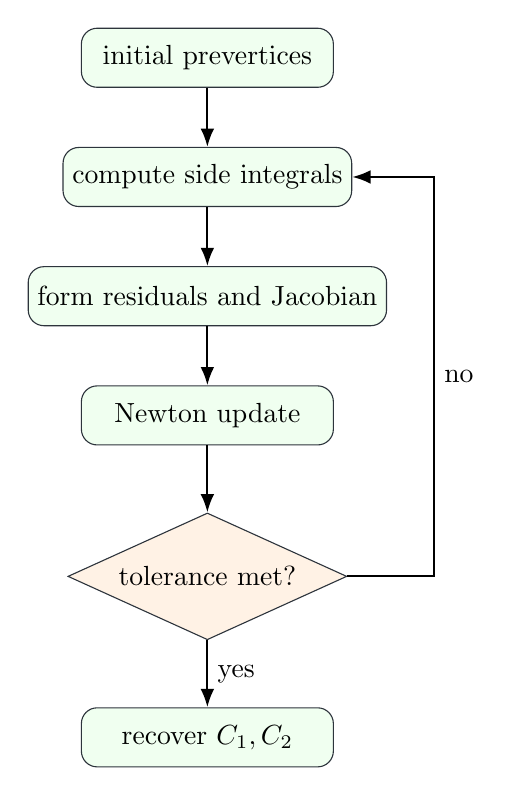
\begin{tikzpicture}[
  block/.style={rectangle,rounded corners=2mm,draw=ink,fill=green!6,align=center,minimum width=3.2cm,minimum height=0.75cm},
  decision/.style={diamond,aspect=2.2,draw=ink,fill=orange!10,align=center},
  arrow/.style={-Latex,thick}
]
\node[block] (guess) {initial prevertices};
\node[block,below=0.75cm of guess] (ints) {compute side integrals};
\node[block,below=0.75cm of ints] (res) {form residuals and Jacobian};
\node[block,below=0.75cm of res] (update) {Newton update};
\node[decision,below=0.85cm of update] (test) {tolerance met?};
\node[block,below=0.85cm of test] (done) {recover \(C_1,C_2\)};
\draw[arrow] (guess) -- (ints);
\draw[arrow] (ints) -- (res);
\draw[arrow] (res) -- (update);
\draw[arrow] (update) -- (test);
\draw[arrow] (test) -- node[right]{yes} (done);
\draw[arrow] (test.east) -- ++(1.1,0) |- node[pos=0.25,right]{no} (ints.east);
\end{tikzpicture}
\caption{Newton iteration for matching side ratios in a polygon.}
\end{figure}

\subsection{Quadrilateral Case}

For a quadrilateral, three of the four prevertices can be fixed by normalization. The remaining prevertex can be represented by a single real parameter \(k\), often chosen so that the four prevertices have a simple ordered form. The side-ratio condition becomes one scalar equation:
\[
F(k)=I_4(k)-\lambda I_1(k)=0.
\]
The update is
\begin{formulabox}
\[
k_{m+1}=k_m-\frac{F(k_m)}{F'(k_m)}.
\]
\end{formulabox}
This case is computationally important because many polygonal domains can be decomposed into quadrilateral-like blocks.

\begin{figure}[H]
\centering
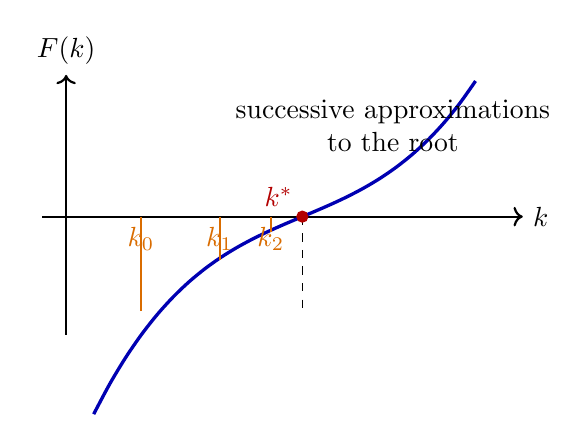
\begin{tikzpicture}[scale=1.0]
\draw[->,thick] (-0.3,0) -- (5.8,0) node[right] {$k$};
\draw[->,thick] (0,-1.5) -- (0,1.8) node[above] {$F(k)$};
\draw[domain=0.35:5.2,smooth,variable=\x,blue!70!black,very thick]
  plot ({\x},{0.075*(\x-3)^3+0.42*(\x-3)});
\draw[dashed] (3,0) -- (3,-1.25);
\filldraw[red!70!black] (3,0) circle (2pt) node[above left] {$k^*$};
\foreach \x/\y/\lab in {0.95/-1.2/$k_0$,1.95/-0.55/$k_1$,2.6/-0.2/$k_2$}{
  \draw[orange!85!black,thick] (\x,\y) -- (\x,0) node[below] {\lab};
}
\node[align=center] at (4.15,1.15) {successive approximations\\to the root};
\end{tikzpicture}
\caption{The quadrilateral parameter problem reduces to scalar root finding.}
\end{figure}

\subsection{Representative Numerical Integral}

A representative side integral in the Schwarz-Christoffel construction is
\begin{formulabox}
\[
L_k = |w_{k+1}-w_k| = |C_1| \int_{x_k}^{x_{k+1}} \left| \prod_{j=1}^{n} (\zeta-x_j)^{-\alpha_j} \right| d\zeta.
\]
\end{formulabox}
The numerical task is to evaluate such integrals accurately. Since the integrand behaves like $|\zeta-x_k|^{-\alpha_k}$ near the left endpoint and $|\zeta-x_{k+1}|^{-\alpha_{k+1}}$ near the right endpoint, it possesses algebraic singularities at both ends of the integration interval. This is why quadrature accuracy and prevertex placement cannot be separated in practical computation.

\begin{figure}[H]
\centering
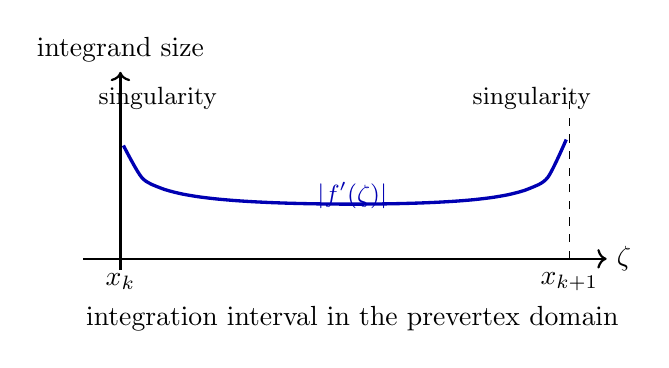
\begin{tikzpicture}[scale=0.95]
\draw[->,thick] (-0.5,0) -- (6.5,0) node[right] {$\zeta$};
\draw[->,thick] (0,-0.15) -- (0,2.5) node[above] {integrand size};
\draw[very thick,blue!70!black,domain=0.04:5.96,smooth,variable=\x]
  plot ({\x},{0.4+0.35/(\x+0.1)^0.55+0.3/(6.1-\x)^0.65});
\draw[dashed] (0.0,0) -- (0,2.2);
\draw[dashed] (6.0,0) -- (6.0,2.2);
\node at (0, -0.3) {$x_k$};
\node at (6, -0.3) {$x_{k+1}$};
\node at (0.5,2.15) {\small singularity};
\node at (5.5,2.15) {\small singularity};
\node[blue!70!black] at (3.1,0.85) {\small $|f'(\zeta)|$};
\node[align=center] at (3.1,-0.8) {integration interval in the prevertex domain};
\end{tikzpicture}
\caption{Repeated SC integral evaluations require quadrature adapted to endpoint singularities.}
\end{figure}

\section{Disk Formulation and Trefethen-Type Algorithms}

An alternative form maps the unit disk to the polygon. If \(z_k=e^{i\Theta_k}\) are prevertices on the unit circle, then
\begin{formulabox}
\[
w(z)=w_c+C\int_0^z\prod_{k=1}^{N}
\left(\frac{z'}{z'-z_k}\right)^{-\alpha_k}\,dz'.
\]
\end{formulabox}
This formulation replaces real prevertex locations by angular unknowns \(\Theta_k\). Numerical algorithms combine nonlinear updates with quadrature rules adapted to algebraic endpoint singularities.

\begin{figure}[H]
\centering
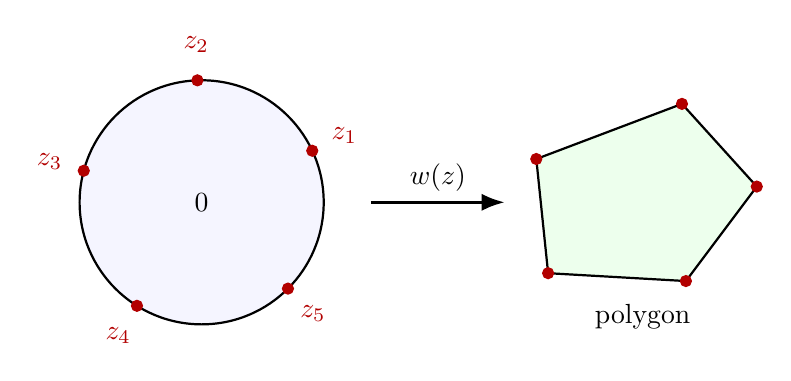
\begin{tikzpicture}[scale=1.0]
\draw[thick,fill=blue!4] (0,0) circle (1.55);
\foreach \a/\lab in {25/$z_1$,92/$z_2$,165/$z_3$,238/$z_4$,315/$z_5$}{
  \filldraw[red!70!black] (\a:1.55) circle (2pt) node at (\a:2.0) {\lab};
}
\node at (0,0) {$0$};
\draw[-Latex,very thick] (2.15,0) -- (3.85,0) node[midway,above] {$w(z)$};
\begin{scope}[xshift=5.6cm]
\draw[thick,fill=green!7] (-1.2,-0.9) -- (0.55,-1.0) -- (1.45,0.2) -- (0.5,1.25) -- (-1.35,0.55) -- cycle;
\foreach \p in {(-1.2,-0.9),(0.55,-1.0),(1.45,0.2),(0.5,1.25),(-1.35,0.55)}{
  \filldraw[red!70!black] \p circle (2pt);
}
\node at (0,-1.45) {polygon};
\end{scope}
\end{tikzpicture}
\caption{Unit-disk SC formulation with prevertices on \(|z|=1\).}
\end{figure}

\begin{figure}[H]
\centering
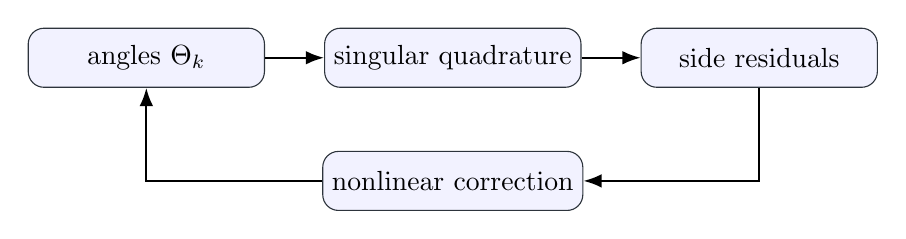
\begin{tikzpicture}[
  block/.style={rectangle,rounded corners=2mm,draw=ink,fill=blue!5,align=center,minimum width=3cm,minimum height=0.75cm},
  arrow/.style={-Latex,thick}
]
\node[block] (ang) {angles \(\Theta_k\)};
\node[block,right=0.75cm of ang] (quad) {singular quadrature};
\node[block,right=0.75cm of quad] (res) {side residuals};
\node[block,below=0.8cm of quad] (upd) {nonlinear correction};
\draw[arrow] (ang) -- (quad);
\draw[arrow] (quad) -- (res);
\draw[arrow] (res) |- (upd);
\draw[arrow] (upd) -| (ang);
\end{tikzpicture}
\caption{Coupling between quadrature and nonlinear parameter updates in disk-based algorithms.}
\end{figure}

\section{Extremal Principles}

An important approach to constructing conformal maps is through extremal principles. The idea, due to Gaier, is to characterize the conformal mapping of a simply connected region \(D\) onto a disk as the solution of a minimization problem in a Hilbert space of analytic functions. Once the minimizer is found, the map follows by integration.

\subsection{Minimum Area Problem}

The conformal mapping of a simply connected domain \(D\) onto a disk can be characterized through a variational principle known as the \textit{Bieberbach minimizing principle}. Rather than specifying the boundary correspondence explicitly, this approach identifies the derivative of the Riemann mapping function as the unique solution to a norm-minimization problem in \(L^2(D)\).

\subsubsection{Function Classes and the Minimization Problem}

Fix a base point \(a \in D\). Define two classes of square-integrable analytic functions:
\[
K_1(D) = \bigl\{ f \in L^2(D) : f \text{ is analytic}, \ f(a) = 1 \bigr\}, \qquad K_0(D) = \bigl\{ f \in L^2(D) : f \text{ is analytic}, \ f(a) = 0 \bigr\}.
\]
Note that the classes \(K_1(D)\) and \(K_0(D)\) represent, respectively, a closed convex subset and a closed subspace of \(L^2(D)\). Let the function
\[
w = f(z) = \sum_{n=0}^{\infty} a_n\,(z - a)^n, \qquad |z - a| < R,
\]
which is regular in \(D\), map \(D\) conformally onto the disk \(B(0,R)\) in the \(w\)-plane. Without loss of generality, we will sometimes take the point \(a\) as the origin.

We will designate the minimum area problem as Problem I, defined as follows:

\begin{formulabox}
\textbf{Problem I:} In the class \(K_1\), minimize the integral
\[
I = \iint_D |f'(z)|^2\,dS_z.
\]
\end{formulabox}

The Riemann mapping theorem guarantees the existence and uniqueness of the solution of this extremal problem.

\begin{theorembox}
\textbf{Theorem (minimum area problem):} Problem I has a unique solution \(f_0(z) = f'(z)\). The minimum is \(\pi R^2\).
\end{theorembox}

\textit{Proof.} Let \(f(z)\) be a mapping function as in the power series above, normalized such that \(f(a) = 0\) and \(f'(a) = 1\). Then the area of the mapped region \(D\) is:
\begin{align*}
\mathrm{area}(D) = \iint_{B(0,R)} |f'(z)|^2 \, dS_z
&= \int_0^R\!\int_0^{2\pi} \bigl|f'(re^{i\theta})\bigr|^2\, r\,dr\,d\theta \\
&= \pi R^2|a_1|^2 + \pi\sum_{n=2}^{\infty} n\,|a_n|^2 R^{2n}.
\end{align*}
The above result implies that for a mapping function regular in the disk and normalized such that \(f'(a) = a_1\), the area of the mapped region is always \(\ge \pi R^2|a_1|^2\). It is exactly equal to this value if the map is linear. For the normalized case \(a_1 = 1\), the minimum area is \(\pi R^2\), and the unique solution to the minimization problem is \(f_0(z) = f'(z)\).

\begin{figure}[H]
\centering
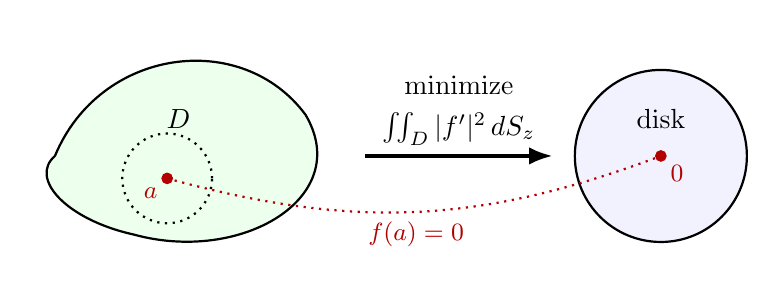
\begin{tikzpicture}[scale=0.95]
% Domain D (back on LHS)
\draw[thick,fill=green!7] (0,0) .. controls (0.6,1.45) and (2.5,1.7) .. (3.35,0.55)
  .. controls (4.0,-0.55) and (2.5,-1.45) .. (1.05,-1.05)
  .. controls (0.15,-0.85) and (-0.35,-0.3) .. (0,0);
\node at (1.65,0.5) {$D$};
\filldraw[red!70!black] (1.5,-0.3) circle (2pt) node[below left,font=\small] {$a$};
\draw[thick, dotted] (1.5,-0.3) circle (0.6);

% Main minimization arrow (pointing from D to Disk)
\draw[-Latex,very thick] (4.15,0) -- (6.65,0) node[midway,above,align=center] {minimize\\[1mm] $\iint_D |f'|^2\,dS_z$};

% Target Disk (back on RHS)
\draw[thick,fill=blue!5] (8.1,0) circle (1.15);
\node at (8.1,0.5) {disk};
\filldraw[red!70!black] (8.1,0) circle (2pt) node[below right,font=\small] {$0$};

% Normalization mapping (dotted line, no arrowhead)
\draw[dotted, thick, red!70!black] (1.5,-0.3) to[bend right=18] node[midway,below,font=\small] {$f(a)=0$} (8.1,0);
\end{tikzpicture}
\caption{The Bieberbach minimizing principle: the derivative of the Riemann map uniquely minimizes the area integral over \(K_1(D)\).}
\end{figure}

\newpage

\begin{theorembox}
\textbf{Theorem (Orthogonality).} The minimizer \(f_0\) is orthogonal in \(L^2(D)\) to every \(g \in K_0(D)\):
\[
\langle f_0,\, g \rangle = \iint_D f_0(z)\,g(z)\,dS_z = 0.
\]
\end{theorembox}

\textit{Proof.} For any \(g \in K_0(D)\) and \(\varepsilon > 0\), the function \(f_0 + \varepsilon g\) lies in \(K_1(D)\) since its value at \(a\) is still 1. By minimality:
\begin{align*}
\|f_0\|^2 &\le \|f_0 + \varepsilon g\|^2 = \|f_0\|^2 + 2\varepsilon\,\Re\langle f_0,g\rangle + \varepsilon^2\|g\|^2.
\end{align*}
Dividing by \(\varepsilon\) and letting \(\varepsilon \to 0^+\) forces \(\Re\langle f_0,g\rangle \ge 0\). Repeating with \(-\varepsilon\) gives the reverse inequality, and replacing \(g\) by \(ig\) settles the imaginary part. Hence \(\langle f_0, g\rangle = 0\).

\subsubsection{Connection to the Bergman Kernel}

Substituting \(g = f - f(a)\) (which belongs to \(K_0(D)\)) into the orthogonality relation gives, for every \(f \in L^2(D)\):
\[
\iint_D f_0(z)\,\overline{f(z)}\,dS_z = f(a)\cdot\|f_0\|^2.
\]
Defining the \textit{Bergman kernel} \(K(z,a) = f_0(z)/\|f_0\|^2\), this becomes the reproducing property
\[
\iint_D K(z,a)\,\overline{f(z)}\,dS_z = f(a), \qquad \text{for all } f \in L^2(D).
\]
Setting \(K(a,a) = 1/\|f_0\|^2\), the minimizer and the conformal map are then recovered as:
\begin{formulabox}
\[
f_0(z) = \frac{K(z,a)}{K(a,a)}, \qquad f(z) = \frac{1}{K(a,a)}\iint_D K(z,a)\,dS_z.
\]
\end{formulabox}
Since \(f_0 = f'\), the conformal mapping function itself is obtained by integrating \(f_0\) from the base point \(a\). In practice, \(K(z,a)\) is not known analytically, but it can be approximated by orthonormalizing a polynomial basis in \(L^2(D)\), which reduces the entire mapping problem to finite-dimensional linear algebra.

\begin{importantbox}
The Bieberbach principle converts the conformal mapping problem into a norm minimization over \(K_1(D)\). The boundary of \(D\) need not be parametrized; only integrals over the domain interior are required to build the Bergman kernel and recover the map.
\end{importantbox}





\subsection{Bergman Kernel Method}

The Bergman kernel method approximates \(K(z,a)\) through a complete orthonormal system \(\{\varphi_j^*(z)\}\) in the analytic \(L^2(D)\) space:
\begin{formulabox}
\[
K(z,a)=\sum_{j=1}^{\infty}\overline{\varphi_j^*(a)}\,\varphi_j^*(z).
\]
\end{formulabox}
In computation, the series is truncated after orthonormalizing a finite basis, often by Gram--Schmidt or an equivalent matrix factorization. The result is an approximate kernel \(K_N(z,a)\), then an approximate minimal function
\[
f_{0,N}(z)=\frac{K_N(z,a)}{K_N(a,a)}.
\]
This approach emphasizes approximation of the reproducing kernel first and then recovers the map from the kernel representation.

\begin{figure}[H]
\centering
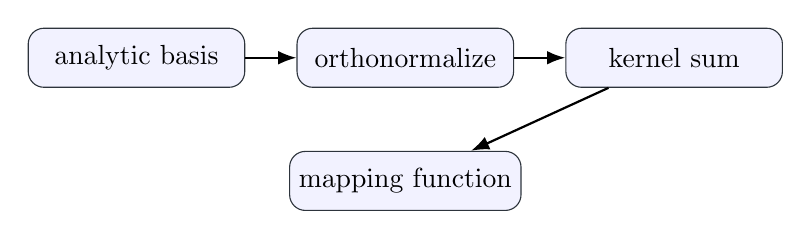
\begin{tikzpicture}[
  block/.style={rectangle,rounded corners=2mm,draw=ink,fill=blue!5,align=center,minimum width=2.75cm,minimum height=0.75cm},
  arrow/.style={-Latex,thick}
]
\node[block] (basis) {analytic basis};
\node[block,right=0.65cm of basis] (orth) {orthonormalize};
\node[block,right=0.65cm of orth] (kernel) {kernel sum};
\node[block,below=0.8cm of orth] (map) {mapping function};
\draw[arrow] (basis) -- (orth);
\draw[arrow] (orth) -- (kernel);
\draw[arrow] (kernel) -- (map);
\end{tikzpicture}
\caption{Bergman kernel method: build an orthonormal basis, approximate the kernel, then recover the map.}
\end{figure}










\section{Applications}

\subsection{Potential Theory}

Electrostatic potential, steady heat conduction, and ideal incompressible flow all lead to Laplace-type equations in two dimensions. A conformal map can move the problem from a complicated geometry to a simple canonical domain, where boundary data are easier to impose.

\begin{figure}[H]
\centering
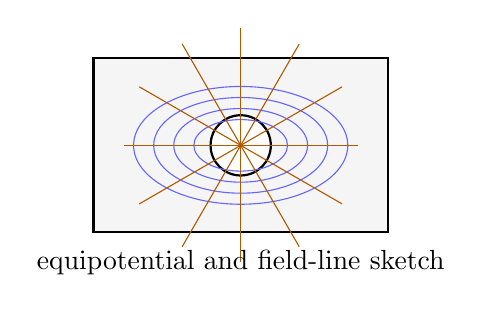
\begin{tikzpicture}[scale=0.85]
\draw[thick,fill=gray!8] (-2.2,-1.3) rectangle (2.2,1.3);
\draw[thick,fill=white] (0,0) circle (0.45);
\foreach \r in {0.7,1.0,1.3,1.6}{
  \draw[blue!60] (0,0) ellipse ({\r} and {0.55*\r});
}
\foreach \a in {0,30,...,330}{
  \draw[orange!70!black,thin] (0,0) -- (\a:1.75);
}
\node at (0,-1.75) {equipotential and field-line sketch};
\end{tikzpicture}
\caption{Conformal maps transfer potential fields between simple and complicated domains.}
\end{figure}

\subsection{Fluid Flow}

For irrotational incompressible flow, the complex potential \(F=\phi+i\psi\) combines velocity potential and stream function. Streamlines and equipotential curves remain orthogonal under conformal maps, allowing flow around difficult boundaries to be studied through a simpler mapped geometry.

\begin{figure}[H]
\centering
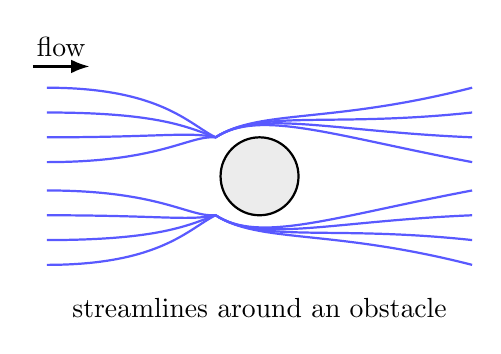
\begin{tikzpicture}[scale=0.9]
\draw[thick,fill=gray!15] (0,0) circle (0.55);
\foreach \y in {-1.25,-0.9,-0.55,-0.2,0.2,0.55,0.9,1.25}{
  \draw[blue!65,thick] (-3,\y) .. controls (-1.4,\y) and (-1.0,{0.55*sign(\y)+0.15*\y}) .. (-0.62,{0.55*sign(\y)})
  .. controls (0,{0.95*sign(\y)}) and (1.0,{0.55*sign(\y)+0.15*\y}) .. (3,\y);
}
\draw[-Latex,thick] (-3.2,1.55) -- (-2.4,1.55) node[midway,above] {flow};
\node at (0,-1.85) {streamlines around an obstacle};
\end{tikzpicture}
\caption{Potential-flow patterns can be generated by mapping canonical flows.}
\end{figure}

\subsection{Computational Grid Generation}

Boundary-fitted orthogonal grids improve numerical simulation near complicated boundaries. A conformal map naturally creates orthogonal coordinate curves, making it useful for mesh generation in polygonal regions.

\begin{figure}[H]
\centering
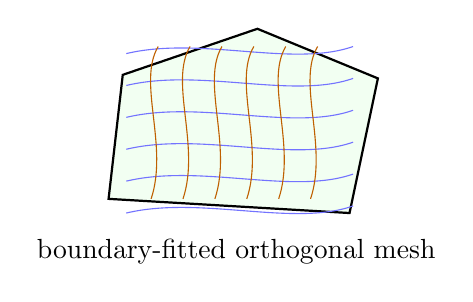
\begin{tikzpicture}[scale=0.9]
\draw[thick,fill=green!5] (-1.8,-1.0) -- (1.6,-1.2) -- (2.0,0.7) -- (0.3,1.4) -- (-1.6,0.75) -- cycle;
\foreach \t in {-1.2,-0.75,-0.3,0.15,0.6,1.05}{
  \draw[blue!55] (-1.55,\t) .. controls (-0.5,\t+0.25) and (0.8,\t-0.2) .. (1.65,\t+0.1);
}
\foreach \x in {-1.2,-0.75,-0.3,0.15,0.6,1.05}{
  \draw[orange!75!black] (\x,-1.0) .. controls (\x+0.25,-0.25) and (\x-0.2,0.65) .. (\x+0.1,1.15);
}
\node at (0,-1.75) {boundary-fitted orthogonal mesh};
\end{tikzpicture}
\caption{Conformal grids preserve orthogonality while adapting to boundary geometry.}
\end{figure}

\section{Conclusion}

This final report has focused on the computational issues that arise after the Schwarz-Christoffel formula is written down. The formula gives the correct angular structure of a polygonal map, but the actual construction requires solving a nonlinear parameter problem and evaluating singular integrals accurately. Newton iteration, singularity subtraction, disk-based algorithms, local approximations, and modulus-based approaches provide different ways to address this task.

The report also described extremal methods, where conformal maps are characterized through the minimum area principle, with the Bergman kernel providing the core theoretical representation. These approaches complement the Schwarz-Christoffel construction and show that conformal mapping is both an analytic and computational subject.

The practical relevance remains broad: potential theory, ideal fluid flow, heat transfer, and numerical grid generation all benefit from transforming complex domains into simpler canonical ones. For polygonal regions, Schwarz-Christoffel mapping remains one of the most direct and geometrically transparent tools for doing so.

\newpage
\section*{Symbols and References}
\addcontentsline{toc}{section}{Symbols and References}

\begin{table}[H]
\centering
\begin{tabular}{@{}ll@{}}
\toprule
Symbol & Meaning \\
\midrule
\(z=x+iy\) & Source-plane complex variable \\
\(w=u+iv\) & Image-plane complex variable \\
\(f(z)\) & Conformal mapping function \\
\(D\) & Physical domain \\
\(\Gamma\) & Boundary of \(D\) \\
\(x_k\) & Real prevertex in the upper-half-plane formulation \\
\(z_k=e^{i\Theta_k}\) & Unit-circle prevertex in the disk formulation \\
\(w_k\) & Polygon vertex \\
\(\theta_k\) & Interior angle at \(w_k\) \\
\(\alpha_k\) & Exterior-angle parameter, \(1-\theta_k/\pi\) \\
\(C_1,C_2\) & Scaling/rotation and translation constants \\
\(I_k\) & Schwarz-Christoffel side integral \\
\(K(z,a)\) & Bergman kernel \\
\bottomrule
\end{tabular}
\end{table}

\vspace{0.8cm}

\begin{enumerate}[label={[\arabic*]}]
\item Prem K. Kythe, \textit{Handbook of Conformal Mappings and Applications}. CRC Press, 2019.
\item Lloyd N. Trefethen, \textit{Numerical Conformal Mapping}.
\end{enumerate}

\end{document}
